\listoftodos


\chapter{Werkzeuge}
\label{chap:Werkzeuge}
Dieses Kapitel erläutert die erstellten Werkzeuge im Detail. Da die Werkzeuge auf einander aufbauen, werden sie der Reihe nach erläutert. 

	\section{ConvolutionalSecondCriterionAutoenocder}
	\label{sec:SecondCriterionAutoenocder}
	Der SCAE erweitert einen ConvolutionalAutoencoder um ein weiteres Kriterium. Es gibt also zusätzlich zu der Rekonstruktion des Autoencoders einen weiteren Ausgang. Der zweite Ausgang kann wie jeder Ausgang für eine Binärklassifikation, für eine Multiklassifikation oder für eine Regression genutzt werden. In Abbildung \ref{img:SchemaSCAE} ist der schematische Aufbau des SCAE abgebildet. 
	
				
		\begin{figure}[h]
			\centering
			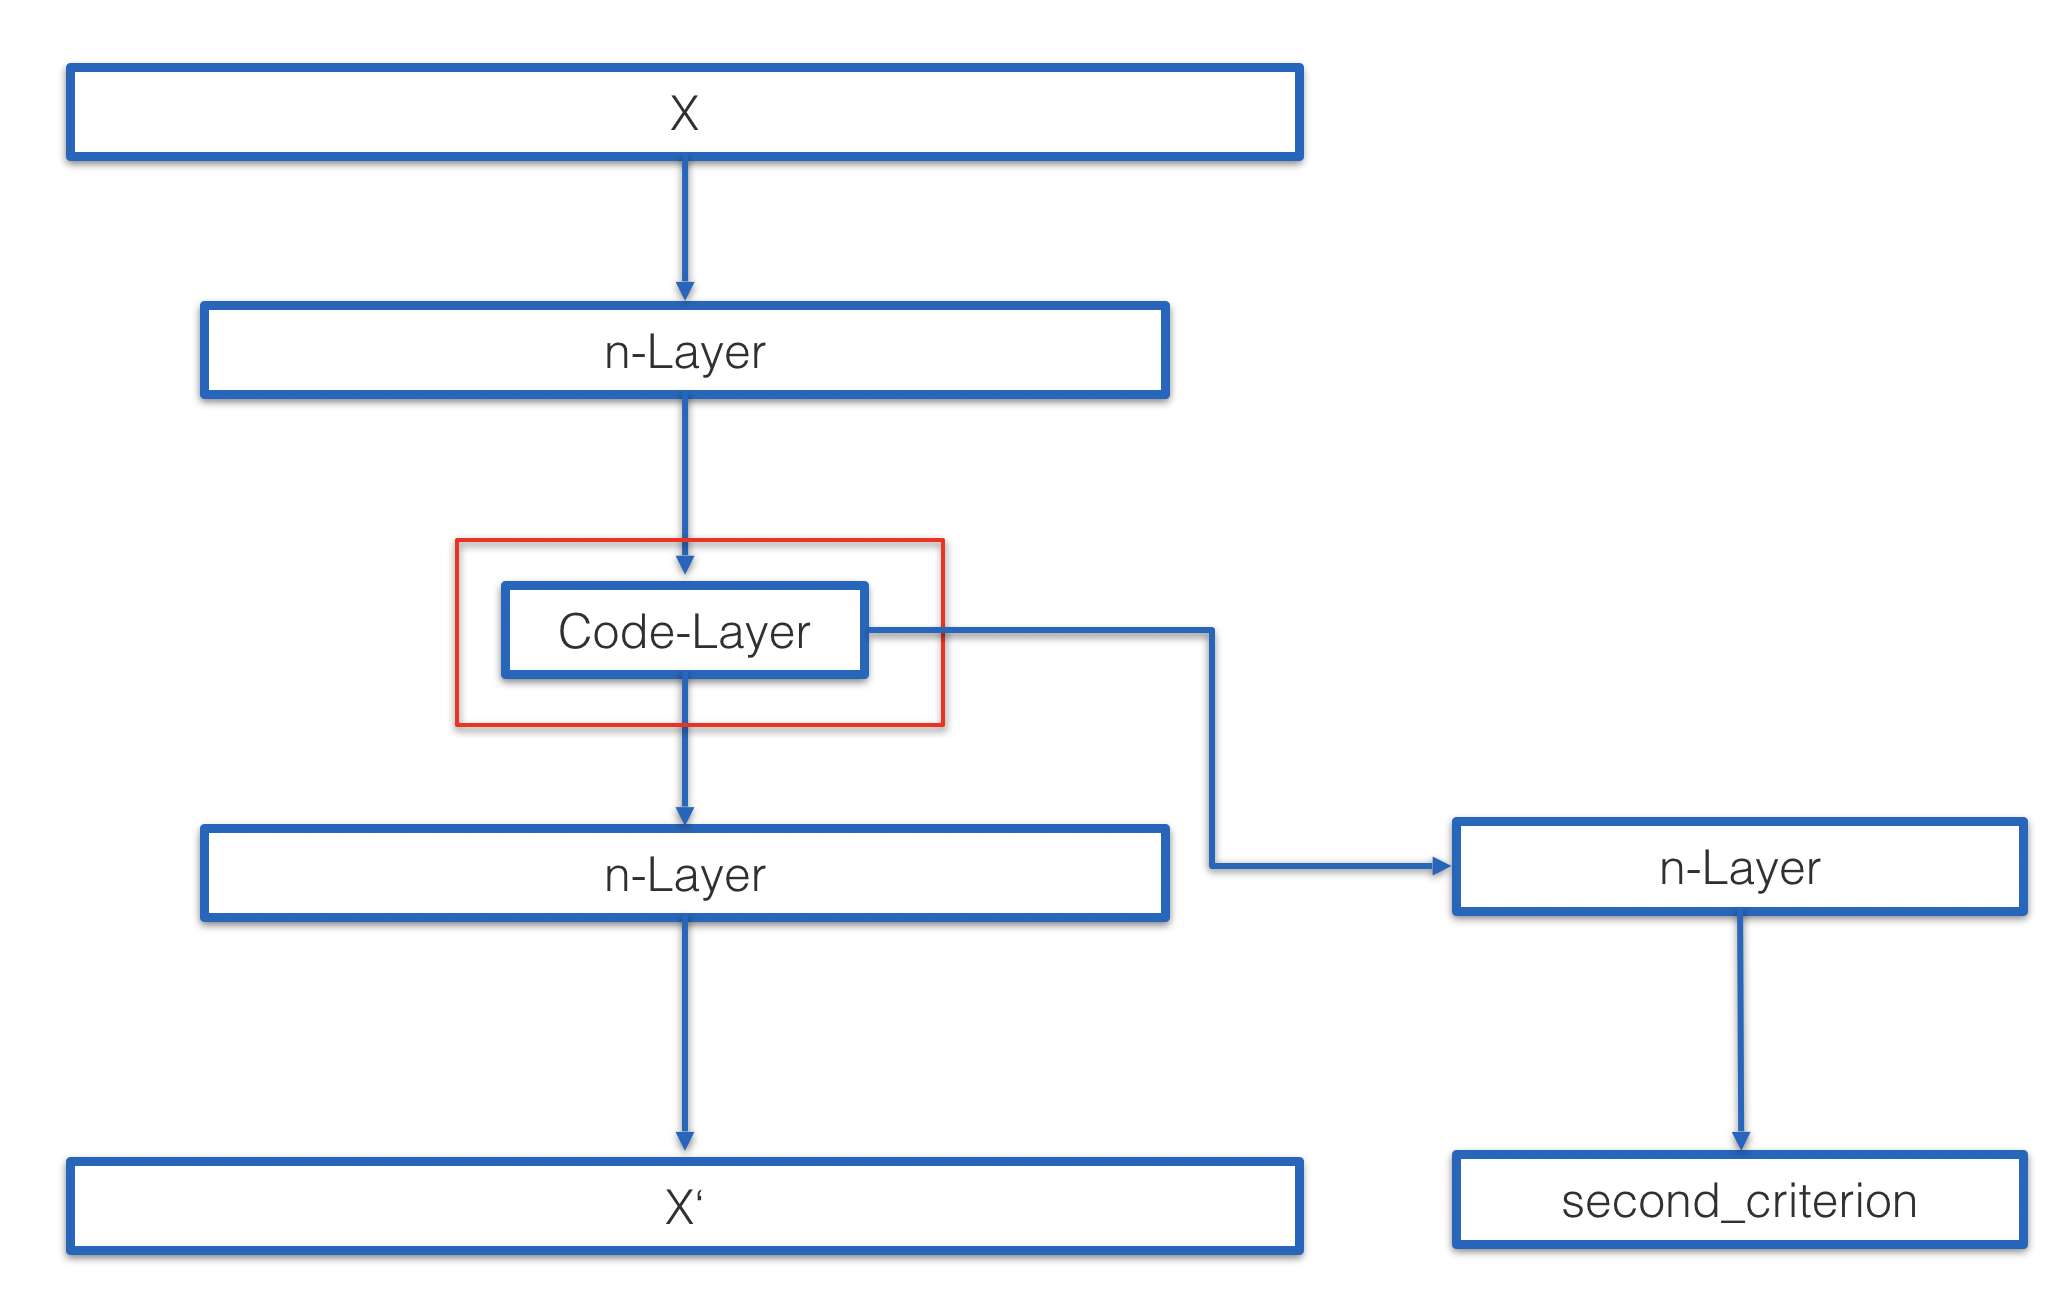
\includegraphics[width=0.5\textwidth, center]{bilder/Schema_Autoencoders/Schema_SCAE.png}
			\caption[Schema SecondCriterionAutoenocder]{Schema SecondCriterionAutoenocder}
			\label{img:SchemaSCAE}
		\end{figure}  
		
		
		\begin{figure}[h]
			\centering
			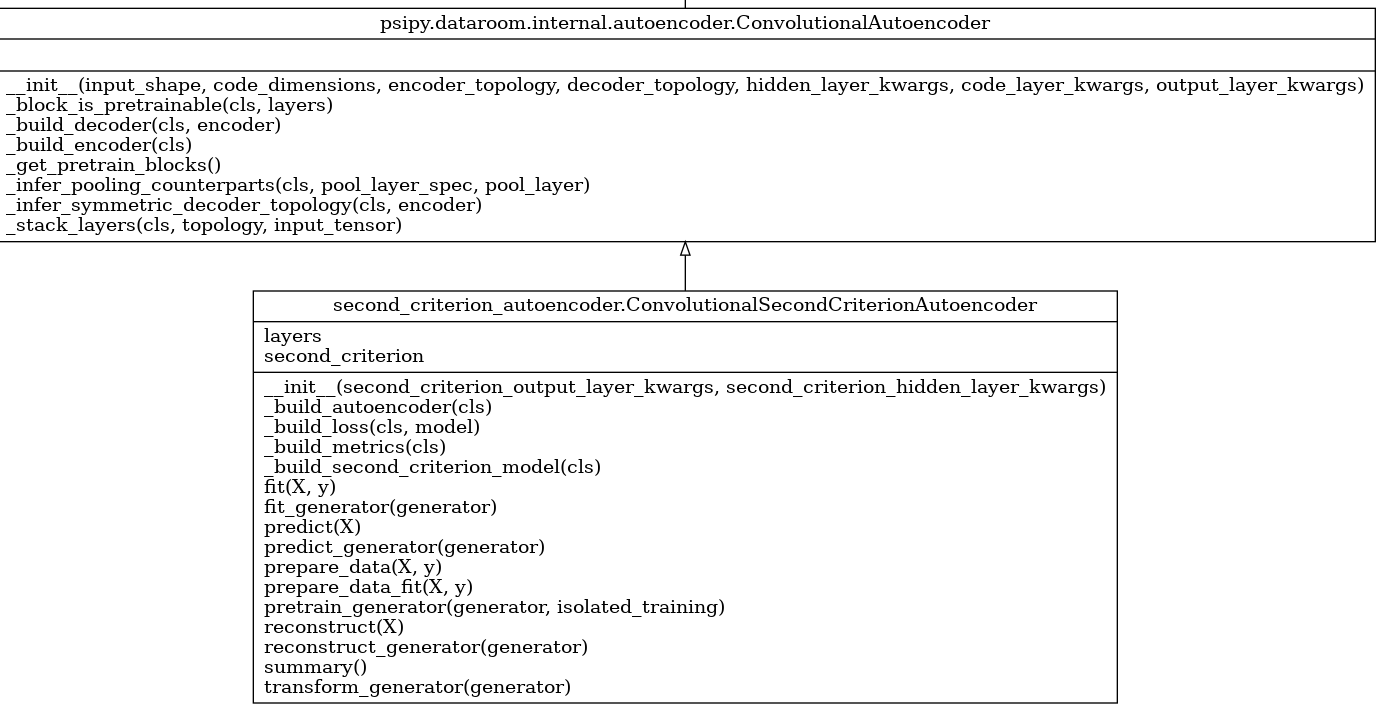
\includegraphics[width=0.5\textwidth, center]{bilder/Klassendiagramme/Klassendiagramm_CSCAE.png}
			\caption[Klassendiagramm ConvolutionalSecondCriterionAutoencoder]{Klassendiagramm ConvolutionalSecondCriterionAutoencoder}
			\label{img:KlassendiagrammCSCAE}
		\end{figure}  
		


	\section{TransferSecondCriterionAutoenocder}
	\label{sec:TransferSecondCriterionAutoenocder}

	\begin{figure}[h]
		\centering
		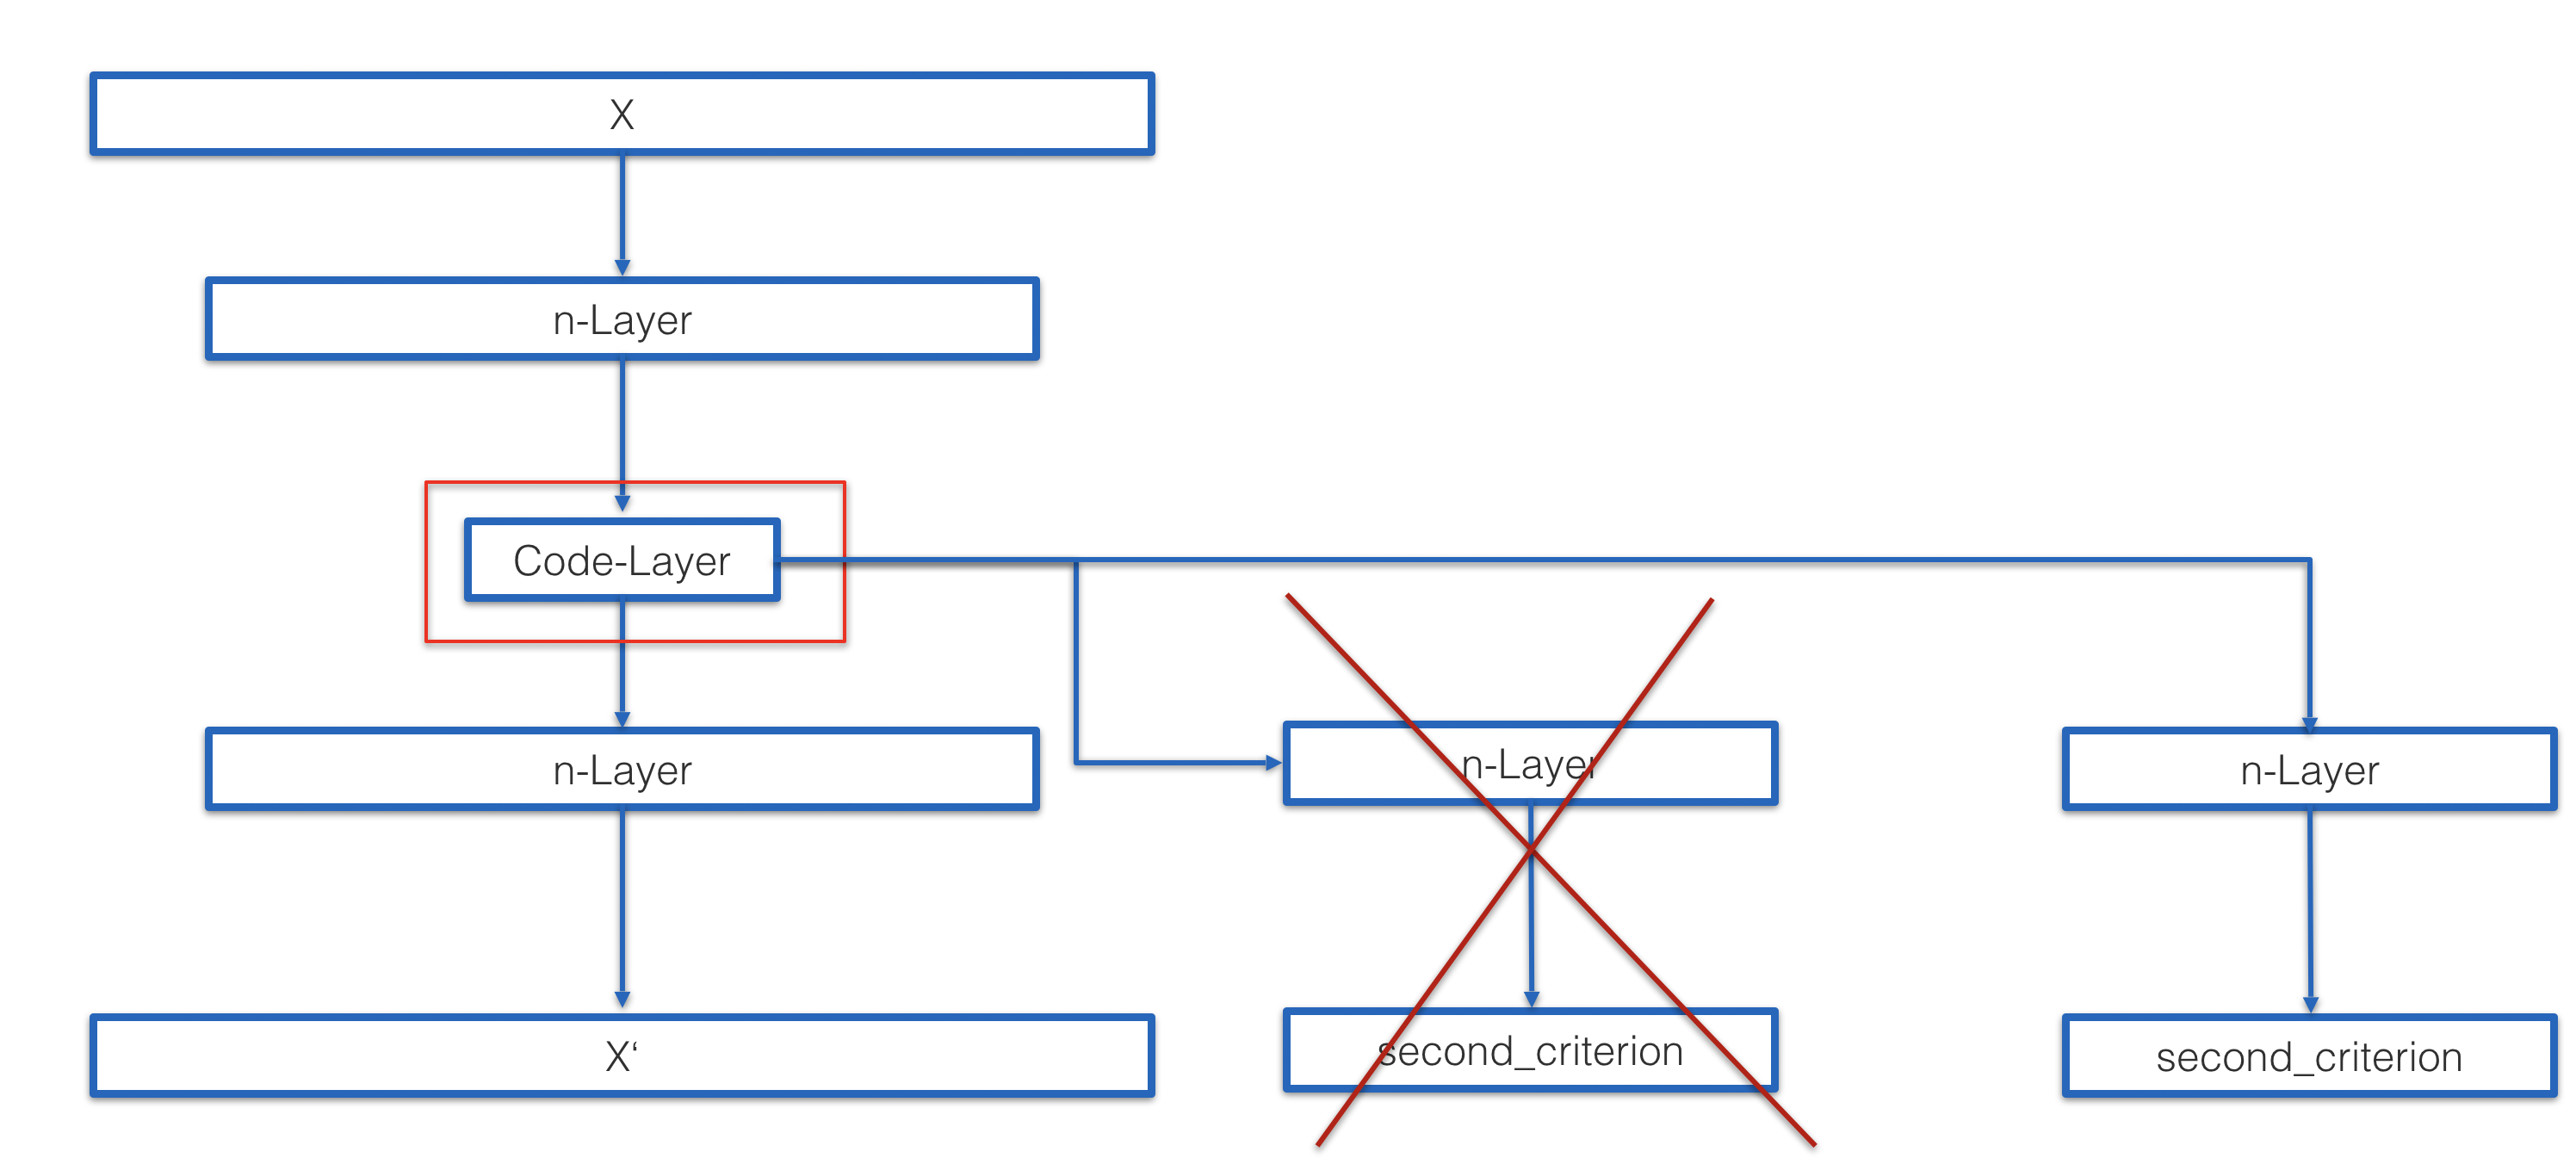
\includegraphics[width=0.5\textwidth, center]{bilder/Schema_Autoencoders/Schema_TSCAE.png}
		\caption[Schema TransferSecondCriterionAutoenocder]{Schema TransferSecondCriterionAutoenocder}
		\label{img:SchemaTSCAE}
	\end{figure}  

	
	\begin{figure}[h]
		\centering
		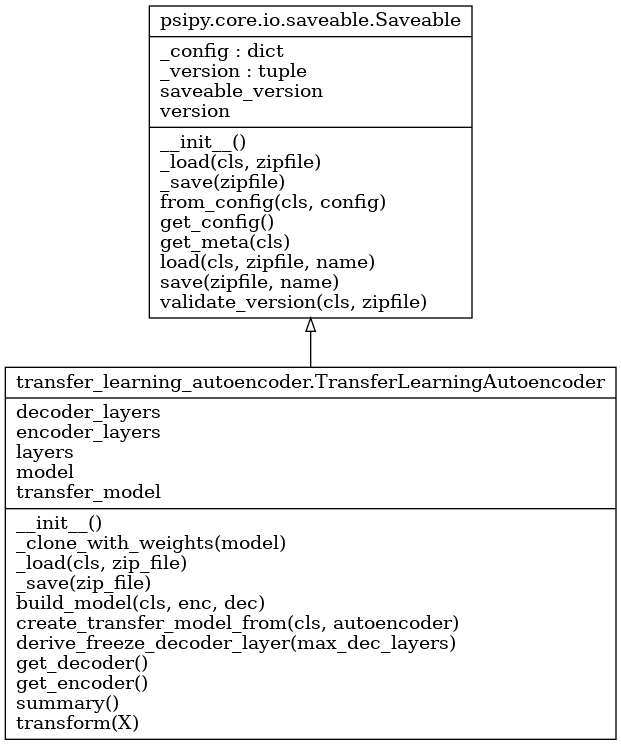
\includegraphics[width=0.5\textwidth, center]{bilder/Klassendiagramme/Klassendiagramm_TLCSCAE.png}
		\caption[Klassendiagramm TransferSecondCriterionAutoenocder]{Klassendiagramm TransferSecondCriterionAutoenocder}
		\label{img:KlassendiagrammTransferSecondCriterionAutoenocder}
	\end{figure}  
			
	\section{AutoTransferSecondCriterionAutoenocder}
	\label{sec:AutoTransferSecondCriterionAutoenocder}


	\begin{figure}[h]
		\centering
		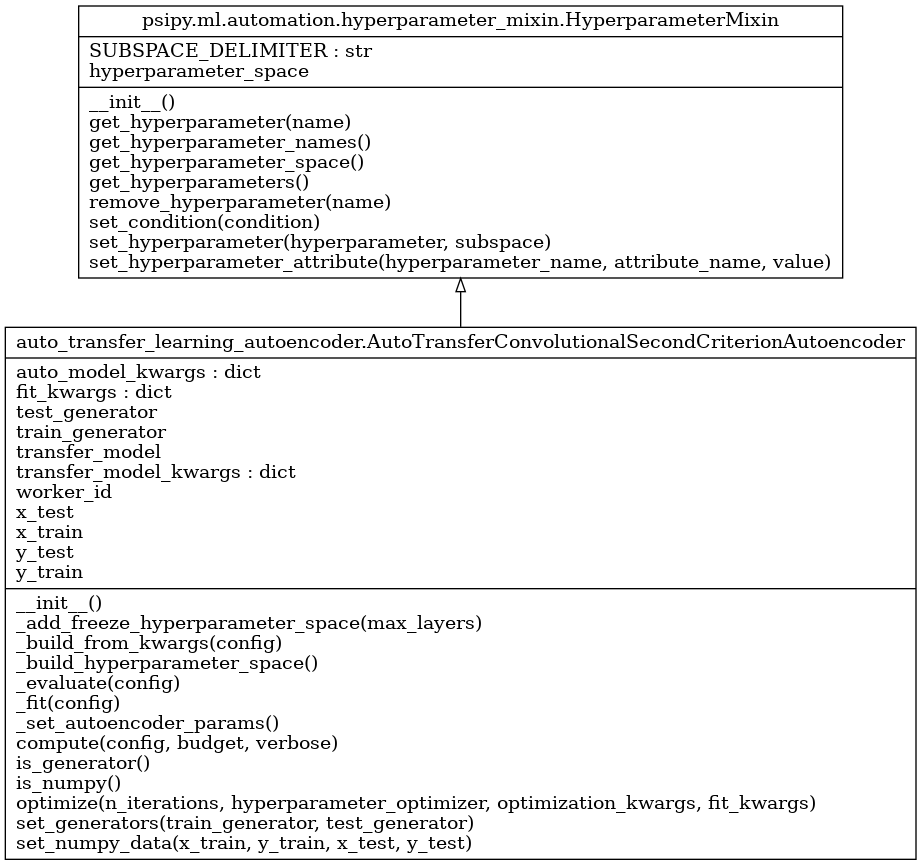
\includegraphics[width=0.5\textwidth, center]{bilder/Klassendiagramme/Klassendiagramm_AutoTLCSCAE.png}
		\caption[Klassendiagramm AutoTransferSecondCriterionAutoenocder]{Klassendiagramm AutoTransferSecondCriterionAutoenocder}
		\label{img:KlassendiagrammAutoTransferSecondCriterionAutoenocder}
	\end{figure}  